%++++++++++++++++++++++++++++++++++++++++
% Don't modify this section unless you know what you're doing!
\documentclass[letterpaper,12pt]{article}
\usepackage[utf8]{inputenc}
\usepackage{float}
\usepackage{tabularx} % extra features for tabular environment
\usepackage{amsmath}  % improve math presentation
\usepackage{graphicx} % takes care of graphic including machinery
\usepackage[margin=1in,letterpaper]{geometry} % decreases margins
\usepackage{cite} % takes care of citations
\usepackage[final]{hyperref} % adds hyper links inside the generated pdf file
\usepackage[table,xcdraw]{xcolor}
\hypersetup{
	colorlinks=true,       % false: boxed links; true: colored links
	linkcolor=blue,        % color of internal links
	citecolor=blue,        % color of links to bibliography
	filecolor=magenta,     % color of file links
	urlcolor=blue         
}
%++++++++++++++++++++++++++++++++++++++++


\begin{document}

\title{Práctica 3 - Ruteo}
\author{Matthew Aguerreberry, Natasha Tomattis}
\date{\today}
\maketitle

% \begin{abstract} 
% \end{abstract}


\section{Practica de Ruteo - OSPF}
	\begin{figure}[ht] 
			
		\centering 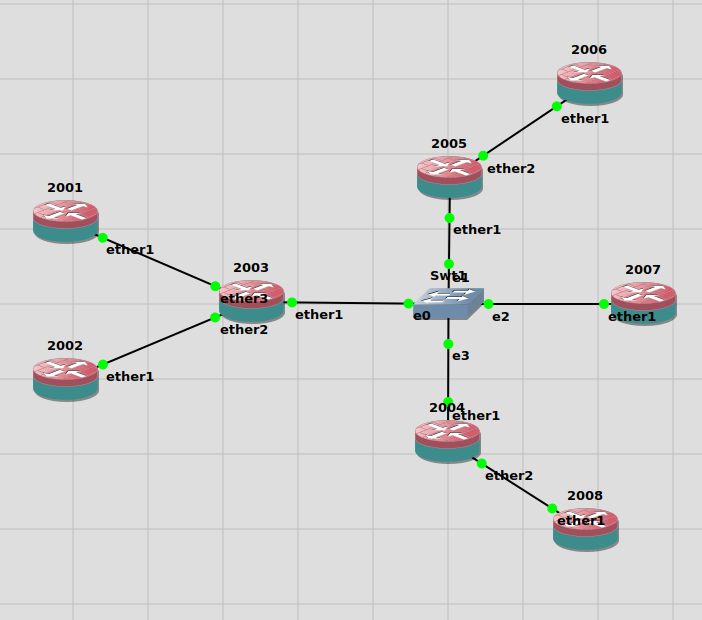
\includegraphics[width=0.8\columnwidth]{figure/topo_figura1.png}
		%\includegraphics[width=1.0\columnwidth]{sr_setup.pdf}
		\caption{
				\label{fig:samplesetup} % spaces are big no-no 
				Implementación Ejercicio 1.
		}
	\end{figure}
	\begin{enumerate}
		\item \textbf{Conectar los routers, switchs y nodos segun el diagrama de la figura 1.}
		\item \textbf{Configurar interfaces de acuerdo al diagrama.}
		\item \textbf{¿Configurar OSPF en todas los routers respetando las areas segun el diagrama. Es posible alcanzar todas las redes?} \\
		Si, todas las redes son compartidas a traves de OSPF.
		\item \textbf{Los routers de las areas no backbone, conocen todas las rutas a las demas redes?}\\
		Si, la division de areas no limita la propagacion de rutas OSPF.
		\item \textbf{Observando el área backbone, que router fue elegido como DR y cual como BDR? ¿Por qué fueron elegidos esos routers?}\\
		Se eligio el router con la router id más alto de la red 10.0.10.0/24 como DR y el subsiguiente como BDR. El router ID, por defecto, toma el valor de IP más bajo de las interfaces activas del dispositivo.
		\item \textbf{Elegir uno de los routers que no cumple una de esas funciones y configurarlo para que sea DR (no debe modificar el direccionamiento) ¿De qué manera/s puede hacer esto? Seleccione una para lograr lo solicitado.}\\
		Esto se puede lograr de varias maneras, por un lado se puede cambiar la prioridad del router la cual sera utilizada a la hora de la eleccion del DR; por otro lado se puede modificar el router-id ya sea a traves de la configuracion explicita de este parametro o la configuracion de una interfaz loopback con una direccion de mayor valar que los otros router-id. En nuestro caso configuramos una interfaz loopback1 en el dispositivo 2003 para que esta sea utilizada como router-id, como se puede ver en la imagen a continuacion.
		\begin{figure}[H] 
			
			\centering 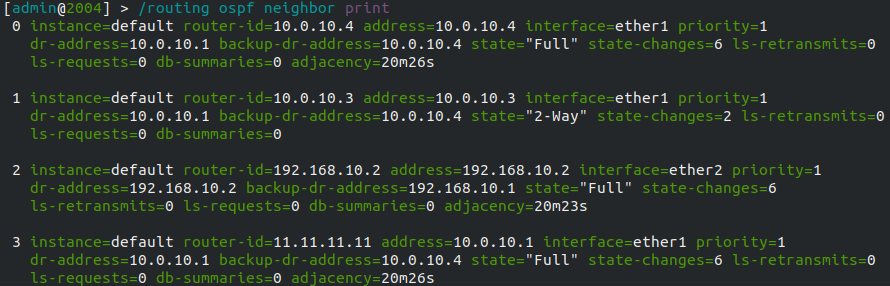
\includegraphics[width=0.5\columnwidth]{figure/int_loopback.png}
			%\includegraphics[width=1.0\columnwidth]{sr_setup.pdf}
			\caption{
					\label{fig:samplesetup} % spaces are big no-no 
					Configuracion de la interfaz loopback en el router 2003.
			}
		\end{figure} 
		\begin{figure}[H] 
			
			\centering 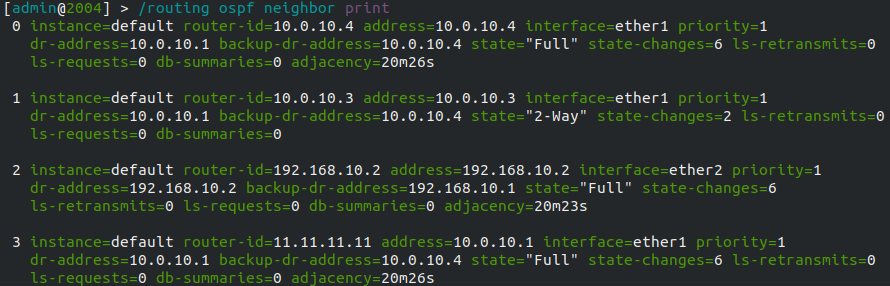
\includegraphics[width=0.8\columnwidth]{figure/new_dr.png}
			%\includegraphics[width=1.0\columnwidth]{sr_setup.pdf}
			\caption{
					\label{fig:samplesetup} % spaces are big no-no 
					Seleccion de la IP configurada en loopback como roter-id. Eleccion de nuevo DR.
			}
		\end{figure}
		\item \textbf{¿Por qué se recomienda definir una dirección de loopback cuando se
		utiliza OSPF?}\\
		Para poder controlar la selección del router-id, y por consiguiente la selección del router designado. Ya que si no se configura una interfaz loopback, esta desición depende de las interfaces configuradas, las cuales pueden cambiar dinamicamente.
		\item \textbf{Explique los distintos tipos de áreas en OSPF}\\
		\item \textbf{En las areas no backbone, ¿también se elige un DR y un BDR?}\\
		Sí.
		\item \textbf{Definir el área 10 como area stub. ¿Qué sucede con la tabla de ruteo
		en el router 2001?}\\
		Se le agraga un default gateway, ya que establecer un área stub impide que el área conozca de rutas externas a OSPF, ete permite el acceso a rutas externas si las hubiera a traves de 2003(ABR). En este caso como todas las rutas aprendidas son por OSPF, no se eliminan entradas en la tabla.
		\begin{figure}[H] 
			
			\centering 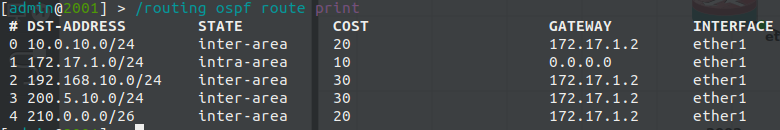
\includegraphics[width=0.7\columnwidth]{figure/routes_default_area.png}
			%\includegraphics[width=1.0\columnwidth]{sr_setup.pdf}
			\caption{
					\label{fig:samplesetup} % spaces are big no-no 
					Rutas en 2001 antes de la configuración como stub area.
			}
		\end{figure} 
		\begin{figure}[H] 
			
			\centering 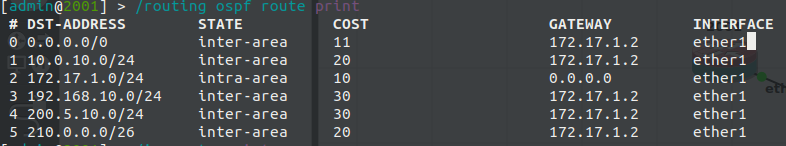
\includegraphics[width=0.7\columnwidth]{figure/routes_stub_area.png}
			%\includegraphics[width=1.0\columnwidth]{sr_setup.pdf}
			\caption{
					\label{fig:samplesetup} % spaces are big no-no 
					Rutas en 2001 después de la configuración como stub area.
			}
		\end{figure}
		\item \textbf{¿Cómo definiría el área 10 para que 2001 solo aprenda de 2003 una ruta default?}\\
		Esto se puede lograr configurando el área 10 como \textit{totally stubby area}, este tipo de configuración impide que se intercambien LSAs de tipo 3 que contienen información sobre las rutas de las otras áreas. El comando utilizado en este caso fue \textit{"/routing ospf area set numbers=1 type=stub inject-summary-lsa=no"}
		\begin{figure}[H] 
			
			\centering 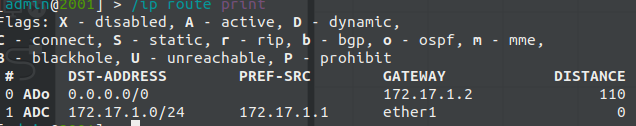
\includegraphics[width=0.7\columnwidth]{figure/routes_totally_stub.png}
			%\includegraphics[width=1.0\columnwidth]{sr_setup.pdf}
			\caption{
					\label{fig:samplesetup} % spaces are big no-no 
					Rutas en 2001 después de la configuración como totally stubby area.
			}
		\end{figure}
		\item \textbf{Seleccionar un router que no sea DR ni BDR y deshabilitar la interface que se conecta contra el área no backbone (por ej. si selecciona el router 2004 deshabilitar la interface ether2). Antes de hacer esto habilitar la captura de paquetes en uno de los enlaces del backbone)}
		
		\item \textbf{¿Qué mensaje envía el router seleccionado en el área backbone? ¿A		quién se lo envía? ¿Qué dirección utiliza? ¿Qué hace el receptor de este mensaje?}\\
		El router envia un mensaje LSA Update, con un LSA de tipo 1 (Router Update) a la dirección multicast 224.0.0.6 (Grupo conformado por DR y BDR). El DR envia el mismo mensaje a la dirccion multicast 224.0.0.5 (Grupo conformado por todos los routers), para que actualicen sus bases de datos.
		\begin{figure}[H] 
			
			\centering 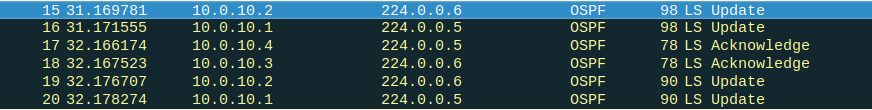
\includegraphics[width=0.7\columnwidth]{figure/2004_ether2_down.png}
			%\includegraphics[width=1.0\columnwidth]{sr_setup.pdf}
			\caption{
					\label{fig:samplesetup} % spaces are big no-no 
					Mensajes en el area backbone luego de deshabilitar una interfaz.
			}
		\end{figure}
		\item \textbf{¿Cómo calcula OSPF el mejor camino a una red? ¿Qué algoritmo
		utiliza?}\\
		El cálculo del mejor camino es en base al ancho de banda de los enlaces, utilizando el algoritmo de Dijkstra.

		\item \textbf{Agregar un nuevo router a la topología según la figura 2}

		\item \textbf{Habilitar OSPF en el nuevo router y enlace agregado}
		
		\item \textbf{En el router 2009, agregar una red loopback, lo0=2.2.2.2/24, y publicarla por OSPF.}
		
		\item \textbf{¿Qué sucede con la tabla de ruteo del router 2002 una vez que se habilita OSPF en la interface ether2? Y 2009, ¿aprende algo por OSPF?}\\
		El router 2002 aprende las rutas del área 169 publicadas por 2009, es decir, las redes 169.192.30.64/28 y 2.2.2.0/24. Por su parte, 2009 aprende las rutas del área 200.
		
		\item \textbf{¿Es posible solucionar esto para que las redes del area 169 sean accesibles desde el resto del dominio OSPF?}\\
		Si, empleando enlaces virtuales que permiten comunicar dos áreas no adyacentes a través de un área de tránsito. Este tipo de áreas necesita dos routers ABRs para pasar tráfico desde un área a otra.\\
		Entonces, el área 200 será de tránsito para comunicar el área 169 con la backbone y de esta manera las redes del area 169 serán accesibles desde el resto del dominio OSPF.
		
		\item \textbf{Agregar un nuevo router a la topologia según la figura 3}

		\item \textbf{Configurar el nuevo enlace y router con RIPv2}
		
		\item \textbf{En el router 2010, agregar una red loopback, lo0=220.0.20.1/24, y publicarla por RIPv2.}
		
		\item \textbf{¿Qué debería hacer el router 2007 para que el dominio OSPF aprenda la red configurada en el paso anterior? ¿Cómo se conocería a ese router en la terminología de OSPF? (Hint.: investigue el concepto de redistribución)}\\
		PREGUNTAR A MARRONE.\\
		En la terminología de OSPF el router 2007 sería conocido como Autonomous System Border Router (ASBR).
		
		\item \textbf{Configurar el router 2007 para que los dos dominios, OSFP y RIPv2, intercambien sus rutas.}
		
		\item \textbf{¿Cómo aprenden las áreas de OSPF esta nueva ruta? ¿Qué sucede en el area 10? Definirla nuevamente como area stub (permitir los summary LSA) y ver si ahora la aprende. ¿Por qué?}\\
		Esta nueva ruta sera aprendida como ruta externa. Solo los routers en la backbone la aprenderán. Por ende, el área 10 debe ser definida como stub utilizando a 2003 como ABR.   
		
		\item \textbf{Capturar tráfico en el área backbone. Deshabilitar y habilitar la interface ether2 de 2007, ¿cómo se publican las redes del entorno RIP? ¿Existe algún LSA de tipo 5? ¿Por qué existe?}\\
		

	\end{enumerate}

	\subsection{Enlaces consultados}
		\begin{itemize}
			\item{HCNA Networking Study Guide}  \\
			\textit{Springer. Huawei Technologies Co., Ltd.},Ch 8.2 RIP.
			\item{Understanding OSPF Stub Areas, Totally Stubby Areas, and Not-So-Stubby Areas}  \\
			\url{https://www.juniper.net/documentation/en_US/junos/topics/concept/ospf-stub-areas-overview.html}
			\item{Manual:Routing/OSPF}  \\
			\url{https://wiki.mikrotik.com/wiki/Manual:Routing/OSPF}
		\end{itemize}
\end{document}